%15 min preso!
\documentclass[xcolor=table,aspectratio=169]{beamer}
\usepackage{beamerthemesplit}
\usepackage{wrapfig}
\usetheme{SPbGU}
\usepackage{pdfpages}
\usepackage{amsmath}
\usepackage{cmap}
\usepackage[T2A]{fontenc}
\usepackage[utf8]{inputenc}
\usepackage[english]{babel}
\usepackage{indentfirst}
\usepackage{amsmath}
\usepackage{tikz}
\usepackage{multirow}
\usepackage[noend]{algpseudocode}
\usepackage{algorithm}
\usepackage{algorithmicx}
\usepackage{fancyvrb}
\usepackage{hyperref} 
\usetikzlibrary{calc}
\usetikzlibrary{shapes, backgrounds}
\usetikzlibrary{arrows,automata}
\usetikzlibrary{positioning}
\usetikzlibrary{fit}
\usetikzlibrary{shapes.callouts}
\usetikzlibrary{shapes.misc}
\usepackage{xparse}
\usepackage{fontawesome}

\usepackage{etoolbox,refcount}
\usepackage{multicol}

\usepackage{tabularx}
\newcolumntype{Y}{>{\raggedleft\arraybackslash}X}

\renewcommand{\thealgorithm}{}

\newtheorem{mytheorem}{Theorem}
\renewcommand{\thealgorithm}{}

\newcommand{\tikzmark}[1]{\tikz[overlay,remember picture] \node (#1) {};}
\def\Put(#1,#2)#3{\leavevmode\makebox(0,0){\put(#1,#2){#3}}}

\newcommand{\ltz}{$< 1$}

\tikzset{
    state/.style={
           rectangle,
           rounded corners,
           draw=black, very thick,
           minimum height=2em,
           inner sep=2pt,
           text centered,
           },
}

\tikzset{
    invisible/.style={opacity=0,text opacity=0},
    visible on/.style={alt=#1{}{invisible}},
    alt/.code args={<#1>#2#3}{%
      \alt<#1>{\pgfkeysalso{#2}}{\pgfkeysalso{#3}} % \pgfkeysalso doesn't change the path
    },
}

\tikzset{cross/.style={cross out, draw=black, minimum size=2*(#1-\pgflinewidth), inner sep=0pt, outer sep=0pt, ultra thick},
%default radius will be 1pt. 
cross/.default={1pt}}

\NewDocumentCommand{\mycallout}{r<> O{opacity=0.8,text opacity=1} m m m}{%
\tikz[remember picture, overlay]\node[align=center, fill=cyan!20, text width=#5cm,
#2,visible on=<#1>, rounded corners,
draw,rectangle callout,anchor=pointer,callout relative pointer={(290:0.5cm)}]
at (#3) {#4};
}

\NewDocumentCommand{\mycalloutR}{r<> O{opacity=0.8,text opacity=1} m m m}{%
\tikz[remember picture, overlay]\node[align=center, fill=cyan!20, text width=#5cm,
#2,visible on=<#1>, rounded corners,
draw,rectangle callout,anchor=pointer,callout relative pointer={(30:0.8cm)}]
at (#3) {#4};
}


%callout relative pointer={(230:0.5cm)}]

\newcounter{countitems}
\newcounter{nextitemizecount}
\newcommand{\setupcountitems}{%
  \stepcounter{nextitemizecount}%
  \setcounter{countitems}{0}%
  \preto\item{\stepcounter{countitems}}%
}
\makeatletter
\newcommand{\computecountitems}{%
  \edef\@currentlabel{\number\c@countitems}%
  \label{countitems@\number\numexpr\value{nextitemizecount}-1\relax}%
}
\newcommand{\nextitemizecount}{%
  \getrefnumber{countitems@\number\c@nextitemizecount}%
}
\newcommand{\previtemizecount}{%
  \getrefnumber{countitems@\number\numexpr\value{nextitemizecount}-1\relax}%
}
\makeatother    
\newenvironment{AutoMultiColItemize}{%
\ifnumcomp{\nextitemizecount}{>}{3}{\begin{multicols}{2}}{}%
\setupcountitems\begin{itemize}}%
{\end{itemize}%
\unskip\computecountitems\ifnumcomp{\previtemizecount}{>}{3}{\end{multicols}}{}}

\definecolor{links}{HTML}{2A1B81}
\hypersetup{colorlinks,linkcolor=,urlcolor=links}


\newcommand\colR{\cellcolor{red!20}}
\newcommand\colB{\cellcolor{blue!20}}
\newcommand\colG{\cellcolor{green!20}}

\beamertemplatenavigationsymbolsempty

\title[Разреженная линейная алгебра: зачем и как]{Обобщённая разреженная линейная алгебра и высокопроизводительный анализ графов в экосистеме RISC-V}
\institute[СПбГУ]{
Санкт-Петербургский Государственный Университет
}

% То, что в квадратных скобках, отображается в левом нижнем углу.
\author[Семён Григорьев]{Семён Григорьев}

\date{18 сентября 2025г.}


%Я предлагаю сначала в общем рассказать интересы и компетенции группы, 
%что научная группа сделала за 3 месяца, 
%потом потратить 1 страницу презентации на каждого из студентов (что сделал, почему важно для Yiming, какие планы). 
%В конце перейти к планам на год.

\begin{document}
{
\begin{frame}[fragile]
  \begin{table}
  \centering
  %
\includegraphics[height=1.5cm]{pictures/SPbGU_Logo.png}
  \begin{tabularx}{\linewidth}{XcX}
    
\includegraphics[height=1.6cm]{pictures/YRS.pdf} \hfill
    & 
    & \hfill 
\includegraphics[height=1.6cm]{pictures/SPbGU_Logo.png}
  \end{tabularx}
  \end{table}
  \titlepage
\end{frame}
}

\begin{frame}[fragile]
  \frametitle{Семён Григорьев}
  \begin{minipage}{0.70\textwidth}
  \begin{itemize}    
    \item Доцент кафедры системного программирования Санкт-Петербургского Государственного Университета
    \item Научный сотрудник лаборатории YADRO
    \item Руководитель исследовательской группы
    \item Области интересов
    \begin{itemize}
      \item \textbf{Высокопроизводительная линейная алгебра} для анализа графов
      \begin{itemize}
        \item \textbf{Обобщённая}: матрицы и вектора параметризованы типом элемента, операции над ними могут быть заданы пользователем
        \item \textbf{Разреженная}: специализированные структуры для хранения матриц и векторов, специализированные алгоритмы для их обработки 
        \item В том числе, с использованием \textbf{графических ускорителей}
      \end{itemize}
      \item \textbf{Высокопроизводительный анализ графов}      
    \end{itemize}
    \end{itemize}
\end{minipage}
\begin{minipage}[t]{0.29\textwidth}
  \begin{center}
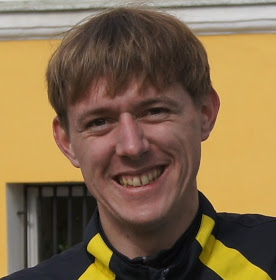
\includegraphics[width=0.8\textwidth]{pictures/SemyonGrigorev.jpg}
  \end{center}
  {\scriptsize
\begin{itemize}    
  \item Email: s.v.grigoriev@mail.spbu.ru
  \item GitHub: \href{https://github.com/gsvgit}{gsvgit}
  \item Google Scholar: \href{https://scholar.google.com/citations?hl=ru&user=kP4dqUAAAAAJ&view_op=list_works&sortby=pubdate}{Semyon Grigorev}
  \item DBLP: \href{https://dblp.org/pid/181/9903.html}{Semyon V. Grigorev}
\end{itemize}
  }
\end{minipage}
\end{frame}

\begin{frame}[fragile]
  \frametitle{Разреженная линейная алгебра}
  \begin{itemize}
    \item Линейная алгебра: матрицы, вектора, операции над ними
    \begin{itemize}
      \item Операции естественным образом распараллеливаются по данным: эффективные реализации для многоядерных систем, GPGPU, и т.д.
      \item Абстракция по операциям: (полу)кольца, моноиды, $\ldots$
    \end{itemize}
    \item \textbf{Разреженная} линейная алгебра: в матрице или векторе много одинаковых элементов
    \begin{itemize}
      \item Часто говорят что в матрице (векторе) много <<нейтральных элементов>>, <<нулей>> или что-то подобное, но это не всегда так
    \end{itemize}
    \item Хотим не хранить одинаковые элементы
    \begin{itemize}
      \item Специальные структуры для хранения матриц и векторов\footnote{COO, CSR, CSC, DCSR, Quad-Tree, $\ldots$}
      \item Специальные алгоритмы для выполнения операций\footnote{Не забываем про параллельность}
    \end{itemize}
  \end{itemize}
\end{frame}


\begin{frame}[fragile]
  \frametitle{Области применения}
  \begin{minipage}{0.46\textwidth}
    \begin{itemize}
    \item Машинное обучение
    \begin{itemize}
      \item Разреженное внимание (sparse attention)
      \item Графовые нейронные сети
    \end{itemize}
    \item Робототехника
    \begin{itemize}
      \item Задачи навигации
      \item $\ldots$
    \end{itemize}
    \item Численные методы
    \begin{itemize}
      \item Разреженные системы уравнений
      \item $\ldots$
    \end{itemize}
    \item $\ldots$
  \end{itemize}
  \end{minipage}
  \begin{minipage}[b]{0.46\textwidth}
    \begin{itemize}
      \item Анализ графов
      \begin{itemize}
        \item Графовые базы данных
        \item Анализ социальных, банковских и других сетей
        \item Статический анализ кода
        \item Биоинформатика
      \end{itemize}
    \end{itemize}
  \end{minipage}
  
\end{frame}

\begin{frame}[fragile]
  \frametitle{Линейная алгебра и анализ графов}
  \begin{itemize}
    \item \textbf{Анализ больших графов}: графовые БД, анализ кода, поиск уязвимостей, анализ трафика, анализ транзакций, банковская аналитика, социальные сети\ldots
      \begin{itemize}
        \item Важна производительность
        \item \underline{\textbf{Разнообразные алгоритмы}}
      \end{itemize}
    \pause  
    \item Путь к унифицированной параллельной обработке графов  
      \begin{itemize}
        \item Граф $\iff$ \textbf{матрица} смежности
        \item Метки на рёбрах $\iff$ \textbf{полукольца}, моноиды, \ldots
        \item Линейная алгебра $\iff$ \textbf{параллелизм} по данным
      \end{itemize}
    \pause  
    \item \textbf{Высокопроизводительная линейная алгебра} для анализа графов
      \begin{itemize}
        \item \textbf{Обобщённая}: матрицы и вектора параметризованы типом элемента, операции над ними могут быть заданы пользователем
        \item \textbf{Разреженная}: специализированные структуры для хранения матриц и векторов, специализированные алгоритмы для их обработки 
        \item В том числе, с использованием \textbf{графических ускорителей}, \textbf{ПЛИС}
      \end{itemize}
    \end{itemize}
\end{frame}

\begin{frame}[fragile]
  \frametitle{GraphBLAS\footnote{\url{https://graphblas.org/}}}
  \begin{itemize}
    \item API для создания алгоритмов анализа графов на основе линейной алгебры 
    \begin{itemize}
      \item Различные операции над матрицами и векторами (\underline{\textbf{разреженными}})
      \item Параметризация алгебраическими структурами: полукольцами, моноидами и т.д.
    \end{itemize}
    \pause
    \item Позволяет выражать \underline{\textbf{различные}} алгоритмы
    \begin{itemize}
      \item Обход в ширину, поиск кратчайших путей, достижимость, \ldots
      \item Подсчёт треугольников, PageRank, остовные деревья, кластеризация,\ldots
      \item Запросы с регулярными (RPQ) и контекстно-свободными (CFPQ) ограничениями \ldots      
    \end{itemize}
    \pause
    \item Подробнее
    \begin{itemize}
      \item The GraphBLAS C API Specification\footnote{\url{https://graphblas.org/docs/GraphBLAS_API_C_v2.1.0.pdf}}
      \item GraphBLAS Pointers\footnote{\url{https://graphblas.org/GraphBLAS-Pointers/}}
      \item Introduction to GraphBLAS\footnote{\url{https://zenodo.org/record/4318870/files/graphblas-introduction.pdf}}
      \item LAGraph\footnote{\url{https://github.com/GraphBLAS/LAGraph}}
    \end{itemize}
    \end{itemize}
\end{frame}

\begin{frame}[fragile]
  \frametitle{Реализации GraphBLAS-подобных API}
  \begin{itemize}
      \item \textbf{SuiteSparse:GraphBLAS}\footnote{\url{https://github.com/DrTimothyAldenDavis/GraphBLAS}}: \underline{\textbf{эталон}} на чистом C
      \item Huawei's GraphBLAS\footnote{\url{https://gitee.com/CSL-ALP/graphblas}}: частичная реализация на C++
      \item CombBLAS\footnote{\url{https://github.com/PASSIONLab/CombBLAS}}: распределённая, частичная реализация на C++
      \item GraphBLAST\footnote{\url{https://github.com/gunrock/graphblast}}: поддержка GPGPU, Cuda C, частичная реализация
      \item Spla\footnote{\url{https://github.com/SparseLinearAlgebra/spla}}: поддержка GPGPU, OpenCL C, частичная реализация
      \item GraphLily\footnote{\href{https://dl.acm.org/doi/10.1109/ICCAD51958.2021.9643582}{GraphLily: Accelerating Graph Linear Algebra on HBM-Equipped FPGAs}}: подмножество GraphBLAS на FPGA
      \item Обёртки для различных языков: Python, Rust, \ldots
      \item \ldots
  \end{itemize}
\end{frame}

\begin{frame}[fragile]
  \frametitle{SuiteStarse\footnote{\url{https://github.com/DrTimothyAldenDavis/SuiteSparse}}}
  \begin{center}
      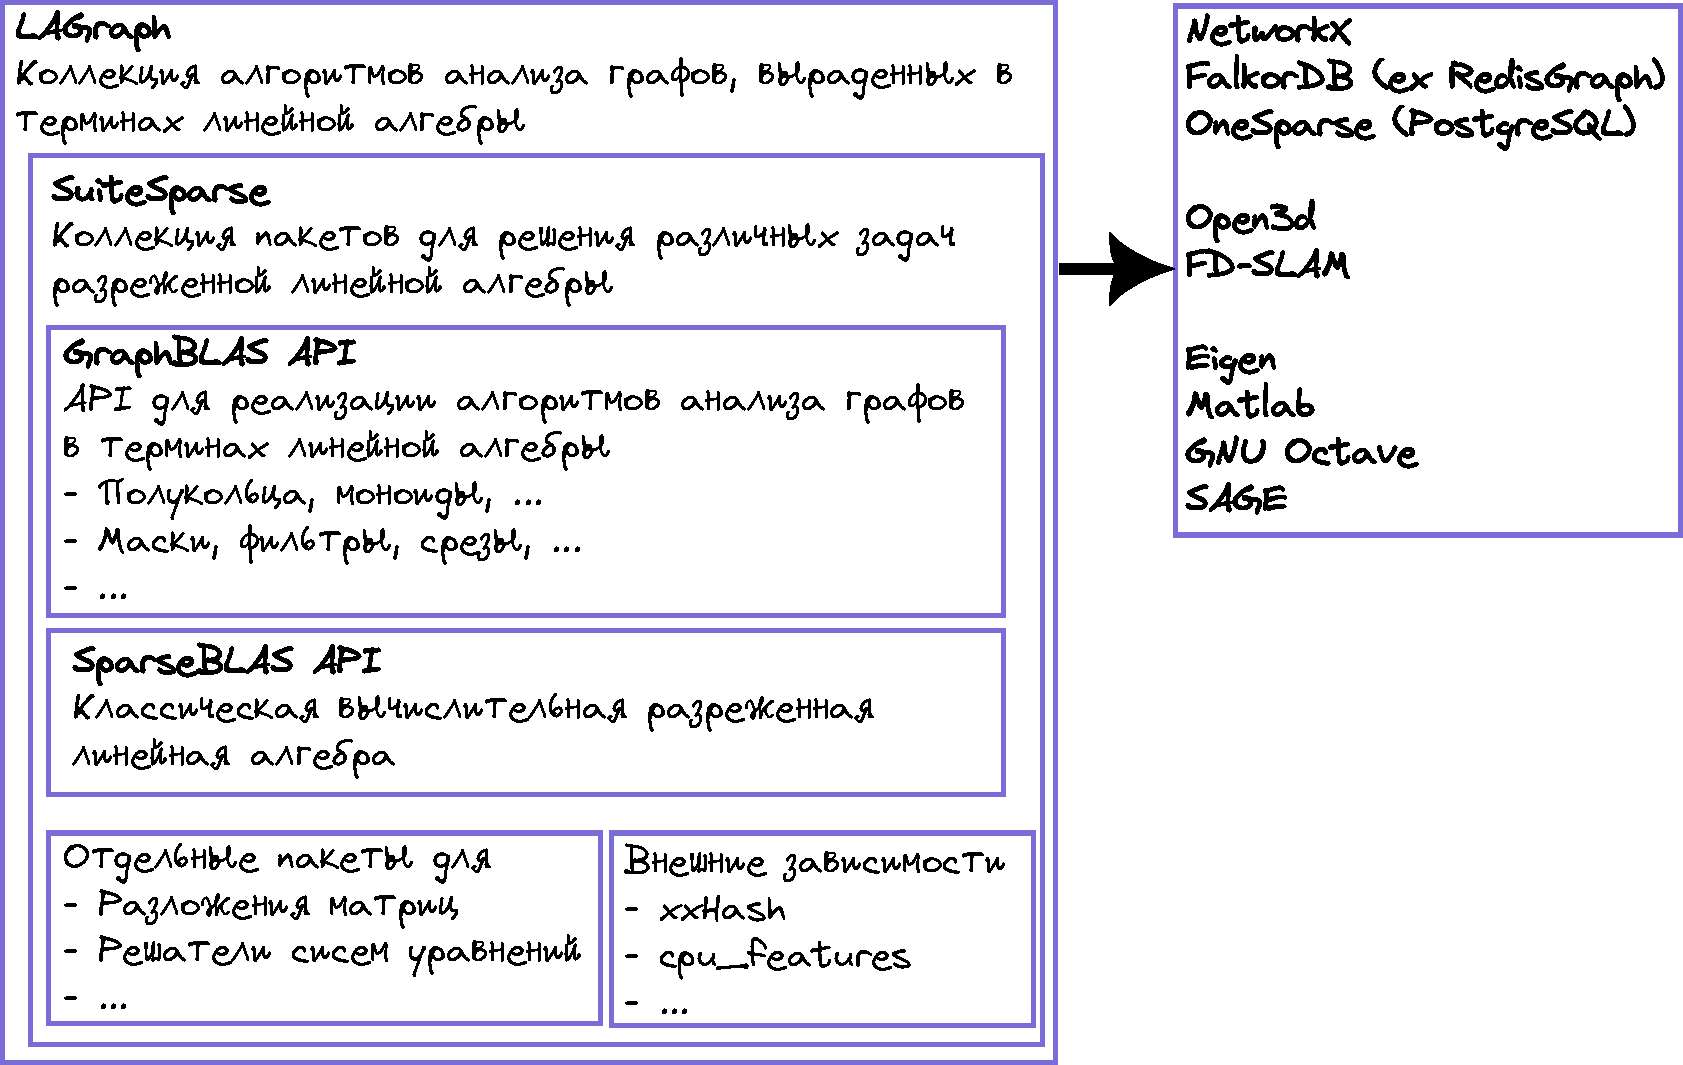
\includegraphics[width=0.68\textwidth]{pictures/SuiteSparse.pdf}
  \end{center}
\end{frame}

\begin{frame}[fragile]
  \frametitle{Пример: обход в ширину}
  \begin{minipage}{0.2\textwidth}
  \begin{tikzpicture}[shorten >=1pt,auto]
    \node[state] (q_0)                      {$0$};
    \node[state] (q_1) [above right=of q_0] {$1$};
    \node[state,fill=red!20] (q_2) [right=of q_0]       {$2$};
    \node[state] (q_3) [right=of q_2]       {$3$};
    \path[->]
    (q_0) edge  node {} (q_1)
    (q_1) edge  node {} (q_2)
    (q_2) edge  node {} (q_0)
    (q_2) edge[bend left, above]  node {} (q_3)
    (q_3) edge[bend left, below]  node {} (q_2);
    \end{tikzpicture}
  \end{minipage}~\pause
  \tikzmark{xPos}{}
  \begin{minipage}{0.75\textwidth}    
    \begin{equation*}
      \left(\begin{array}{cccc}        
        0  & 0  & \colR 1 & 0 \\        
      \end{array}\right)
      \times    
      \left(\begin{array}{cccc}        
        0 & 1 & 0 & 0 \\
        0 & 0 & 1 & 0 \\
        \rowcolor{red!20}
        1 & 0 & 0 & 1 \\
        0 & 0 & 1 & 0 \\        
      \end{array}\right)
      =      
        \left(\begin{array}{cccc}        
          \colB 1 & 0  & 0 & \colB 1 \\        
        \end{array}\right)
    \end{equation*}
    \mycallout<2-4>[opacity=1]{$(xPos) + (2.9,0.4)$}{Текущий фронт}{2.5}
    \mycallout<2-4>[opacity=1]{$(xPos) + (5.9,1.1)$}{Матрица смежности}{3.5}
    \mycallout<2-4>[opacity=1]{$(xPos) + (9.2,0.4)$}{Новый фронт}{2.5}
    \mycalloutR<2-4>[opacity=1]{$(xPos) + (4.3,0.2)$}{Полукольцо}{2.1}
  \end{minipage}

  \pause

  \begin{minipage}{0.2\textwidth}
    \begin{tikzpicture}[shorten >=1pt,auto]
      \node[state, fill=blue!20] (q_0)                      {$0$};
      \node[state] (q_1) [above right=of q_0] {$1$};
      \node[state, fill=red!20] (q_2) [right=of q_0]       {$2$};
      \node[state, fill=blue!20] (q_3) [right=of q_2]       {$3$};
      \path[->]
      (q_0) edge  node {} (q_1)
      (q_1) edge  node {} (q_2)
      (q_2) edge  node {} (q_0)
      (q_2) edge[bend left, above]  node {} (q_3)
      (q_3) edge[bend left, below]  node {} (q_2);
      \end{tikzpicture}
    \end{minipage}~
    \begin{minipage}{0.75\textwidth}
    \begin{equation*}
      \left(\begin{array}{cccc}        
        \colB 1 & 0  & 0 & \colB 1 \\        
      \end{array}\right)
      \times
      \left(\begin{array}{cccc}        
        \rowcolor{blue!20}
        0 & 1 & 0 & 0 \\
        0 & 0 & 1 & 0 \\        
        1 & 0 & 0 & 1 \\
        \rowcolor{blue!20}
        0 & 0 & 1 & 0 \\        
      \end{array}\right)
      =      
        \left(\begin{array}{cccc}        
          0 & \colG 1  & \colG 1 & 0 \\        
        \end{array}\right)
    \end{equation*}
    \pause     
    \begin{tikzpicture}[overlay,remember picture,auto]
        \draw (9.16, 1.21) node[cross=10pt, color=red] {};
    \end{tikzpicture}
  \end{minipage}

\end{frame}


\begin{frame}[t]
  \frametitle{Векторизация умножения матриц в SuiteSparse:GraphBLAS\footnote{Соответствующий PR: \url{https://github.com/DrTimothyAldenDavis/GraphBLAS/pull/381}}}
  \begin{itemize}    
    \item Оборудование
    \begin{itemize}
    \item X86\_64
    \begin{itemize}
  \item \textbf{CPU}: Intel Core i7-12700H 800MHz с векторами размером 1024 битов
  \item \textbf{RAM}: LPDDR4, 16GB
  \item \textbf{Compiler}: GCC 14.2.0
\end{itemize}
    \item RISC-V
    \begin{itemize}
  \item \textbf{SoC}: SPACEMIT K1/M1, Octa-core X60™(RV64GCVB), RVA22, RVV1.0 1600MHz с векторами размером 2048 битов 
  \item \textbf{RAM}: LPDDR4X, 16GB 
  \item \textbf{Compiler}: GCC 14.2.0 (cross)
\end{itemize}
    \end{itemize}
    \item SuiteSparse matrix collection: матрицы разных размеров и разной степени разреженности
    \item Сравнивали изменение величины среднего времени выполнения 400 запусков умножения матриц
  \end{itemize}  
\end{frame}

\begin{frame}[t]
  \frametitle{Результаты экспериментального исследования векторизованного кода\footnote{Во всех экспериментах стандартное отклонение не превосходит 5\%}}
  \begin{center}
    \resizebox{0.9\textwidth}{!}{
    \tikzmark{zzz}{ }
    \begin{tabular}{|p{0.5cm}|p{3.4cm}|p{1.4cm}|p{1.5cm}|p{1.3cm}|p{1.3cm}|p{1.5cm}|p{1.5cm}|p{1.28cm}|p{1.28cm}|}
        \hline
        \textbf{№} & \textbf{Matrix name} & \textbf{Rows number} & \textbf{Nonzeros}& \textbf{AVX2 (ms.)}& \textbf{No AVX2 (ms.)}& \textbf{RVV (ms.)}& \textbf{No RVV (ms.)}& \textbf{AVX speedup (\%)}& \textbf{RVV speedup (\%)} \\
        \hline
        1 & olafu & 16146 & 515651 & 5327.7 & 6629.7 & 43080.7 & 52940.1 & 19.6 & \cellcolor{green!25}18.6 \\
        \hline
        \cellcolor{ red!30}2 & \cellcolor{red!30}fd18 & \cellcolor{red!30}16428 & \cellcolor{red!30}63406 & \cellcolor{red!30}476.4 & \cellcolor{red!30}482.0 & \cellcolor{red!30}2212.6 & \cellcolor{red!30}2181.2 & \cellcolor{red!30}1.2 & \cellcolor{red!50}-1.4 \\
        \hline
        3 & sme3Da & 12504 & 874887 & 4236.9 & 5124.9 & 32008.0 & 42763.8 & 17.3 & \cellcolor{green!25}25.2 \\
        \hline
        4 & stokes64 & 12546 & 74242 & 508.8 & 564.4 & 2629.7 & 2814.1 & 9.8 & \cellcolor{green!25}6.6\\
        \hline
        5 & sinc12 & 7500 & 294986 & 632.6 & 864.0 & 5970.1 & 8593.8 & 26.8 & \cellcolor{green!25}30.5\\
        \hline
        6 & fd12 & 7500 & 28462 & 90.4 & 92.3 & 484.1 & 555.3 & 2.0 & \cellcolor{green!25}12.8\\
        \hline
        7 & bcsstk15 & 3948 & 60882 & 87.8 & 117.9 & 1271.5 & 1770.8 & 25.6 & \cellcolor{green!25}28.2\\
        \hline
        8 & tols4000 & 4000 & 8784 & 17.1 & 18.2 & 184.0 & 203.5 & 5.9 & \cellcolor{green!25}9.6\\
        \hline
        9 & ex36 & 3079 & 53843 & 28.5 & 41.0 & 574.2 & 584.8 & 30.5 & \cellcolor{green!25}1.8\\
        \hline
        10 & iprob & 3001 & 9000 & 25.2 & 34.7 & 279.3 & 344.9 & 27.5 & \cellcolor{green!25}19.0\\
        \hline
        11 & MISKnowledgeMap & 2427 & 28511 & 31.3 & 38.5 & 401.6 & 490.0 & 18.8 & \cellcolor{green!25}18.0 \\
        \hline
        \cellcolor{ red!30}12 & \cellcolor{ red!30}LeGresley\_2508 & \cellcolor{ red!30}2508 &\cellcolor{ red!30}16727 & \cellcolor{ red!30}10.4 & \cellcolor{ red!30}12.1 & \cellcolor{ red!30}106.5 & \cellcolor{ red!30}97.7 & \cellcolor{ red!30}14.3 & \cellcolor{red!50}-8.9\\
        \hline
        13 & reorientation\_2 & 1544 & 9408 & 5.6 & 9.8 & 117.9 & 125.4 & 42.7 & \cellcolor{green!25}6.0\\
        \hline
        \cellcolor{ red!30}14 & \cellcolor{ red!30}netscience & \cellcolor{ red!30}1589 & \cellcolor{ red!30}2742 & \cellcolor{ red!30}1.5 & \cellcolor{ red!30}2.8 & \cellcolor{ red!30}31.4 & \cellcolor{ red!30}28.5 & \cellcolor{ red!30}47.0 & \cellcolor{red!50}-10.0\\
        \hline
        15 & mcfe & 765 & 24382 &2.3 & 5.5 & 51.1 & 65.3 & 58.8 & \cellcolor{green!25}21.8\\
        \hline
        16 & orbitRaising\_3 & 761 & 3256 & 0.6 & 1.6 & 10.5 & 13.1 & 63.0 & \cellcolor{green!25}19.5\\
        \hline

    \end{tabular}
}
  \end{center}
  \onslide<2>{
    \tikz[overlay,remember picture]{\draw[draw=blue,thick,double,fill opacity=0.2] ($ (zzz) + (11.1,0.6)$) rectangle ($ (zzz) + (13.5,0.25)$);}
    \tikz[overlay,remember picture]{\draw[draw=blue,thick,double,fill opacity=0.2] ($ (zzz) + (11.1,1.6)$) rectangle ($ (zzz) + (13.5,1.25)$);}
    }
  \onslide<3>{
    \tikz[overlay,remember picture]{\draw[draw=red,thick,double,fill opacity=0.2] ($ (zzz) + (11.1,-2.45)$) rectangle ($ (zzz) + (13.5,-3.15)$);}
    \tikz[overlay,remember picture]{\draw[draw=red,thick,double,fill opacity=0.2] ($ (zzz) + (11.1,-0.43)$) rectangle ($ (zzz) + (13.5,-0.75)$);}
    \tikz[overlay,remember picture]{\draw[draw=red,thick,double,fill opacity=0.2] ($ (zzz) + (11.1,-1.8)$) rectangle ($ (zzz) + (13.5,-2.14)$);}
    }
\end{frame}

\begin{frame}[fragile]
  \frametitle{Кросс-сборка и тестирование SuiteSparse\footnote{Соответствующий реквекст: \url{https://github.com/DrTimothyAldenDavis/SuiteSparse/pull/949}}}
  \begin{itemize}
    \item \textbf{Было}
    \begin{itemize}
      \item Alpine linux + chroot\footnote{До недавнего времени не было RISC-V}
      \item Сборка и тестирование в эмуляторе (qemu)\footnote{Не для всех компонент}
      \item Продолжительность workflow в GitHub CI: 2 часа 20 минут
    \end{itemize}
    \pause
    \vfill
    \item \textbf{Стало}
      \begin{itemize}
        \item Кросс-тулчейн + MultiArch
        \item Кросс-сборка и тестирование в эмуляторе (qemu-user)\footnote{Для всех компонент}
        \item Продолжительность workflow в GitHub CI: 40 минут
        \item Выявлены и локализованы ошибки под x390s и ppc64le\footnote{Позже выяснилось, что про них знали и ошибка в GCC а не в SuiteSparse}
      \end{itemize}
    \pause
    \item Предложенное нами решение для кросс-сборки начали использовать в GNU Octave\footnote{\url{https://github.com/DrTimothyAldenDavis/SuiteSparse/pull/955\#discussion_r2103092266}}
  \end{itemize}
\end{frame}

\begin{frame}
  \frametitle{Spla на SpacemiT M1 (RISC-V) с IMG BXE-2-32 GPU}

\begin{columns}
        \column{0.5\textwidth}        
        \vspace{-0.5cm}
        \begin{center}
          BFS \\
        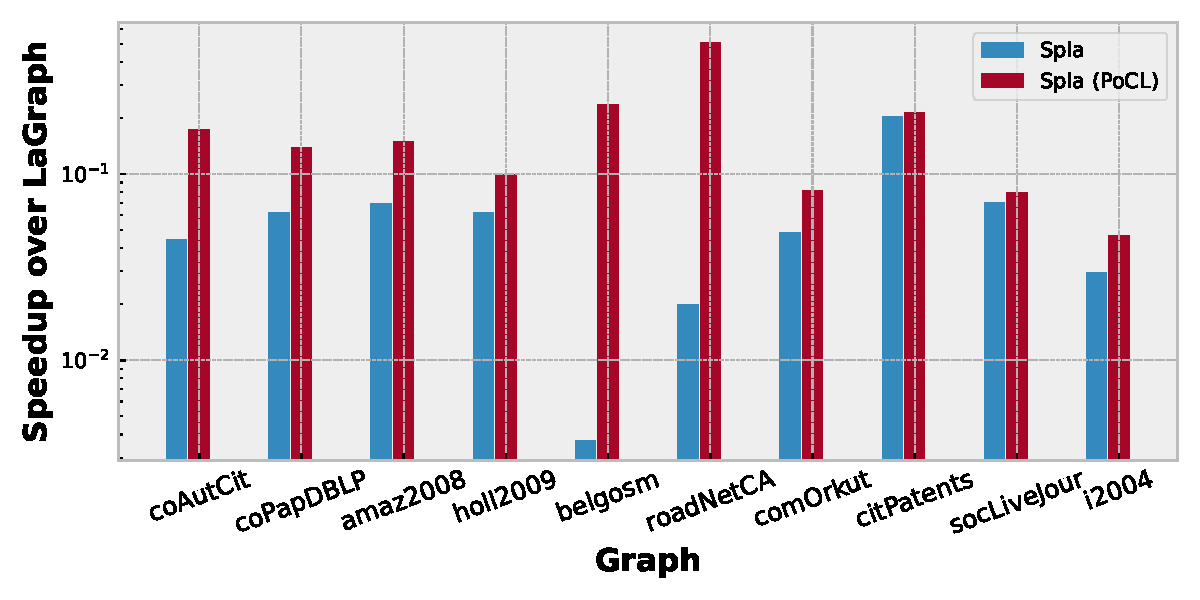
\includegraphics[width=0.909\linewidth]{pictures/rq1_rel_bfs.pdf}
        Single Source Shortest Path (SSSP) \\
        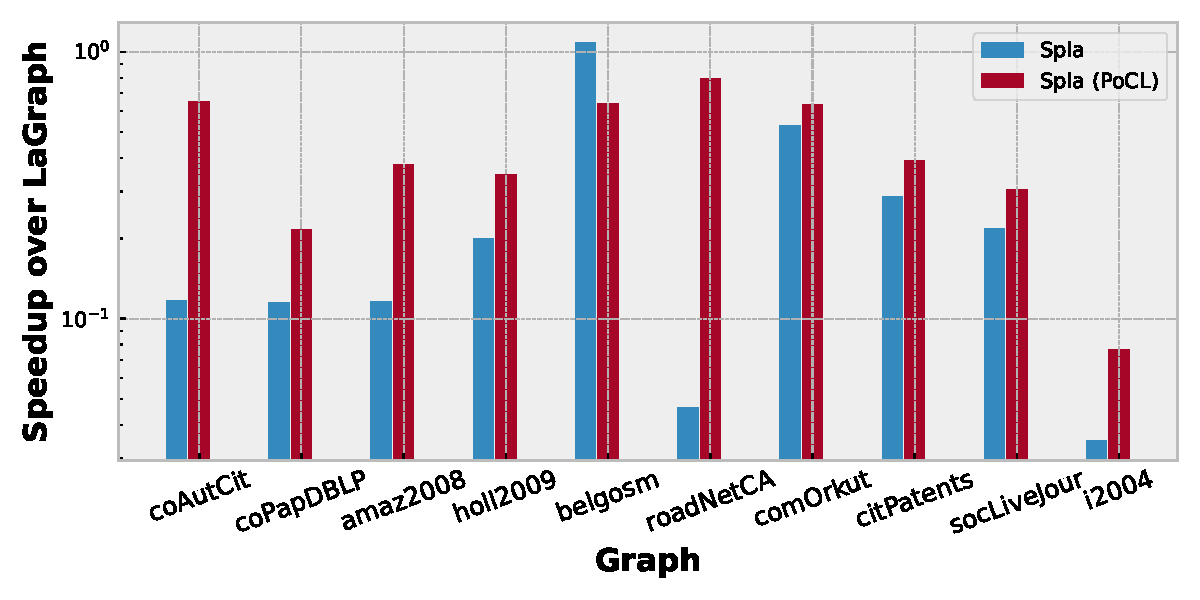
\includegraphics[width=0.909\linewidth]{pictures/rq1_rel_sssp.pdf}
        \end{center}
        \column{0.5\textwidth}
        \vspace{-0.5cm}
        \begin{center}
          Triangle Count (TC) \\
        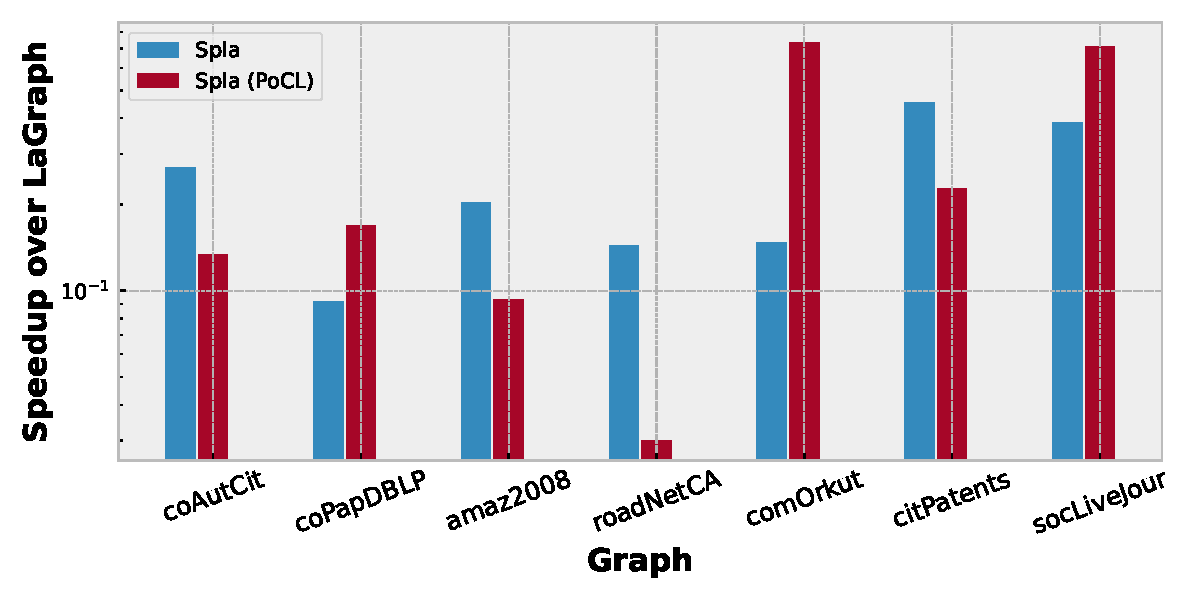
\includegraphics[width=0.9\linewidth]{pictures/rq1_rel_tc.pdf}
        PageRank (PR) \\
        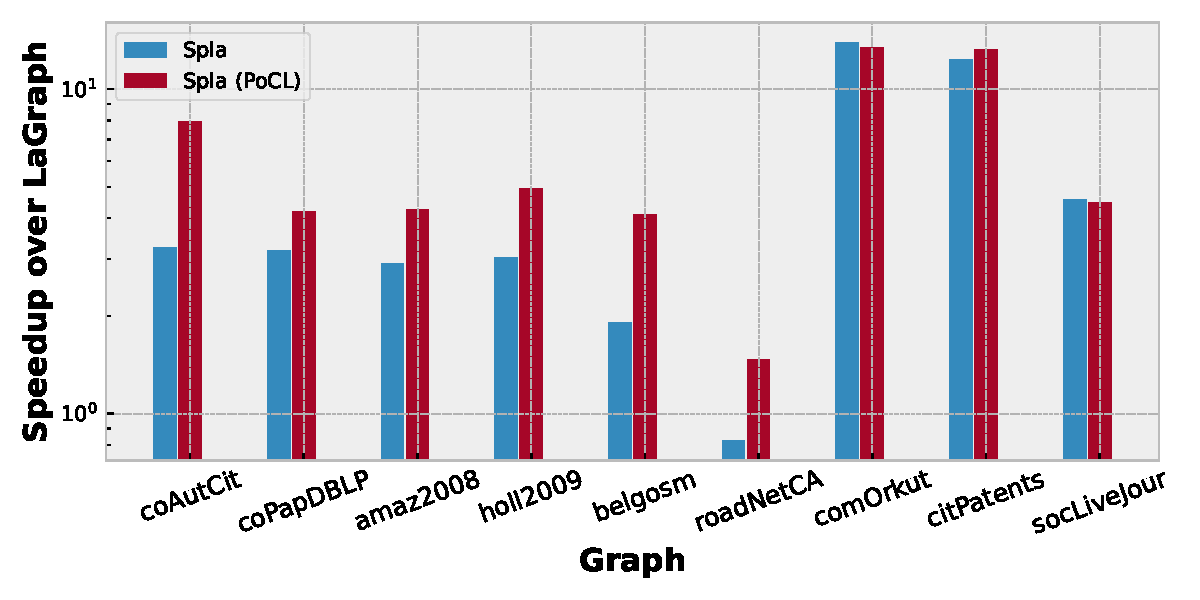
\includegraphics[width=0.9\linewidth]{pictures/rq1_rel_pr.pdf}
        \end{center}
    \end{columns}
    
\end{frame}

\begin{frame}
  \frametitle{Результаты умножения плотных матриц на SpacemiT M1 с IMG GPU}
  \begin{center}
  \tikzmark{z1}{ }
  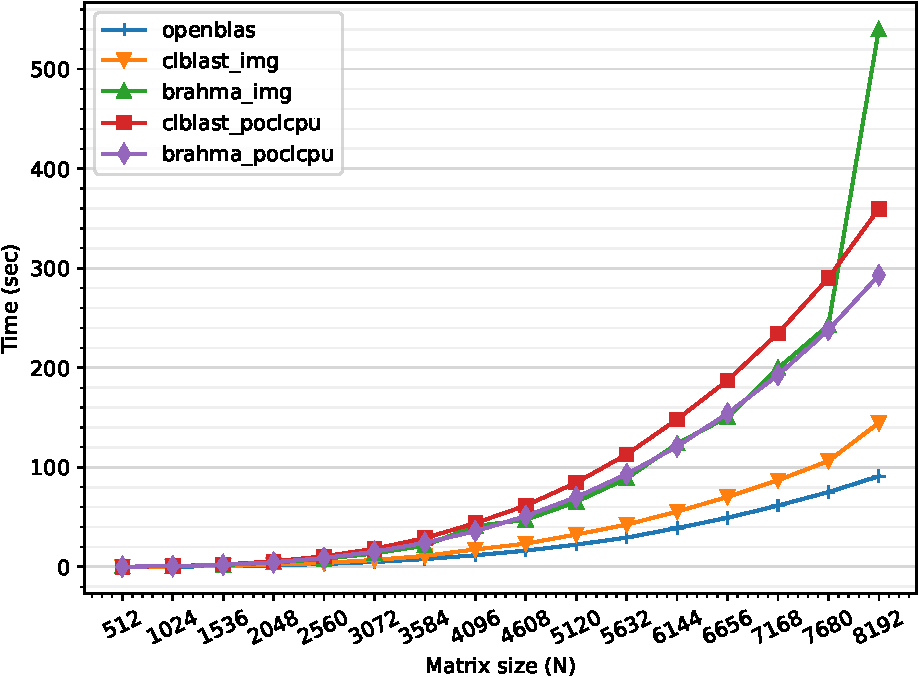
\includegraphics[width=0.55\textwidth]{pictures/MILK-V_crop.pdf}
  \tikz[overlay,remember picture]{\draw[draw=red,thick,double,fill opacity=0.2] ($ (z1) + (1.1,5.45)$) rectangle ($ (z1) + (3.4,6.05)$);}
  \\
    GPGPU от Imagination Technologies (пока) не совсем для вычислений
  \end{center}
\end{frame}

\begin{frame}[fragile]
  \frametitle{Пара слов про \href{https://github.com/vortexgpgpu/vortex}{Vortex}: RISC-V GPGPU}
  \begin{itemize}
    \item Набор инструкций, основанный на RISC-V ISA
    \item Поддержка OpenCL через POCL 
    \begin{itemize}
      \item[\faGears] Spla должен запускаться
    \end{itemize}
    \item Проблемы со сбросом регистров
    \begin{itemize}
      \item Типичные оптимизации не работают
      \item \href{https://github.com/vortexgpgpu/vortex/issues/251}{Issue 1}
      \item \href{https://github.com/vortexgpgpu/vortex/issues/205}{Issue 2}
    \end{itemize}
    \item В целом, есть подозрение, что мало регистров
    \item Для ПЛИС с HBM
    \begin{itemize}
      \item[\faQuestion] Бонус для обработки слабоструктурированных данных
    \end{itemize}
  \end{itemize}
\end{frame}

\begin{frame}[fragile]
  \frametitle{Перспективы: RISC-V}
  \begin{itemize}
    \item Идёт работа над расширениями\footnote{Оставим в покое RVV, Integrated Matrix Extension, XuanTie Matrix Extension, \ldots}   
    \begin{itemize}
      \item \href{https://ieeexplore.ieee.org/abstract/document/10546747}{IndexMAC: A Custom RISC-V Vector Instruction to Accelerate Structured-Sparse Matrix Multiplications}, 2024 год
      \item \href{https://dl.acm.org/doi/abs/10.1007/978-3-031-40843-4_35}{Optimizations for Very Long and Sparse Vector Operations on a RISC-V VPU: A Work-in-Progress}, 2023 год
      \item \href{https://dl.acm.org/doi/10.1109/TC.2025.3533083}{Optimizing Structured-Sparse Matrix Multiplication in RISC-V Vector Processors}, 2025 год
      \item \href{https://ieeexplore.ieee.org/abstract/document/10271722}{Sparse Stream Semantic Registers: A Lightweight ISA Extension Accelerating General Sparse Linear Algebra}, 2023 год
      \item \href{https://ieeexplore.ieee.org/abstract/document/11113397}{Hardware/Software Co-Design of RISC-V Extensions for Accelerating Sparse DNNs on FPGAs}, 2024 год       
    \end{itemize}
    \item В основном для машинного обучения: малая разрядность, относительно большая плотность, фиксированный набор типов и операций (часто для инференса)
    \item Vortex: \href{https://cea.hal.science/cea-05043041v1/document}{GPGPUs on FPGAs: A competitive approach for scientific computing?}, 2025 год
  \end{itemize}
\end{frame}

\begin{frame}[fragile]
  \frametitle{Специализированные решения для разреженной линейной алгебры}
  \begin{itemize}
    \item \href{https://dl.acm.org/doi/10.1145/3640542}{Dedicated Hardware Accelerators for Processing of Sparse Matrices and Vectors: A Survey}, 2024 год
    \item \href{https://dl.acm.org/doi/10.1145/3604606}{A Survey of Accelerating Parallel Sparse Linear Algebra}, 2023 год
    \item \href{https://dl.acm.org/doi/abs/10.1145/3571157}{A Systematic Literature Survey of Sparse Matrix-Vector Multiplication}, 2024 год
  \end{itemize}
\end{frame}


\begin{frame}[fragile]
  \frametitle{Заключение}  
  \begin{itemize}
    \item Высокопроизводительная разреженная линейная алгебра $\Rightarrow$ высокопроизводительные приложения
    \begin{itemize}
      \item Машинное обучение
      \item Графовые базы данных
      \item Анализ социальных, банковских и других сетей
      \item Анализ кода
      \item $\ldots$
    \end{itemize}
    \item Сделать \textbf{разреженную} линейную алгебру высокопроизводительной \textbf{сложно}
    \begin{itemize}
      \item Нерегулярный доступ к данным
      \item Хорошая алгебра --- \textbf{обобщённая} алгебра
      \item Сложности с балансировкой нагрузки
      \item $\ldots$
    \end{itemize}
    \item Но люди пытаются
    \begin{itemize}
      \item Даже институты для этого создают\footnote{Sparsitute: A mathematical Institute for Sparse Computations in Science and Engineering, \href{https://sparsitute.lbl.gov/}{https://sparsitute.lbl.gov/}}
    \end{itemize}
  \end{itemize}
\end{frame}


\end{document}
